%-------------------------------------------------------------------------------
%-------------------------------------------------------------------------------
%-------------------------------------------------------------------------------
\chapter{DS4+ X-ENS 2018}
%-------------------------------------------------------------------------------
%-------------------------------------------------------------------------------
\vskip -2cm
\begin{center}
    \Huge \bf Nombre chromatique \\et coloriage de graphe
\end{center}
%-------------------------------------------------------------------------------
%-------------------------------------------------------------------------------
\section*{Préliminaires}
%-------------------------------------------------------------------------------
%-------------------------------------------------------------------------------
%-------------------------------------------------------------------------------
\subsection*{Complexité}
%-------------------------------------------------------------------------------
Par \emph{complexité en temps} d'un algorithme $A$, on entend le nombre d'opérations élémentaires  (comparaison, addition, soustraction, multiplication, division, affectation, test, etc.) nécessaire à l'exécution de $A$ dans le pire cas. 

Lorsque la complexité en temps dépend d'un ou plusieurs paramètres $k_1, \dots, k_r$, on dit qu'elle est en $O(f(k_1,\dots,k_r))$ s'il existe une constante $C > 0$ telle que, pour toutes les valeurs de $k_1,\dots, k_r$ suffisamment grandes (c'est-à-dire plus grandes qu'un certain seuil), la complexité est au plus $C\times f(k_1,\dots,k_r)$.

On dit que la complexité en temps est \emph{linéaire} quand $f$ est une fonction linéaire des paramètres $k_1, \dots, k_r$, \emph{polynomiale} quand $f$ est une fonction polynomiale des paramètres $k_1, \dots, k_r$, et enfin \emph{exponentielle} quand $f = 2^g$, où $g$ est une fonction polynomiale des paramètres $k_1,\dots,k_r$.

Les complexités (en temps) des algorithmes \emph{devront être justifiées}. 
%-------------------------------------------------------------------------------
\subsection*{Graphes}
%-------------------------------------------------------------------------------
Rappelons qu'un graphe non-orienté est la donnée $(S,A)$ de deux ensembles finis : \begin{itemize} 
    \item  un ensemble $S$ de \emph{sommets}, et
    \item un ensemble $A \subseteq S\times S$ d'\emph{arêtes}, tel que pour tout couple de sommets $(s,t)$, on a $s\ne t$ pour $(s, t) \in A$ et  $(s,t) \in A$ si et seulement si $(t,s) \in A$.
\end{itemize}

Étant donné un graphe $G = (S,A)$, le \emph{sous-graphe induit} par un ensemble de sommets $T \subseteq S$ est $(T,A\cap (T\times T))$. 

Soit $G = (S,A)$ un graphe et soit $s \in S$ un sommet de $G$. Un \emph{voisin} de $s$ est un sommet $t$ de $G$ qui est relié à $s$ par une arête, c'est-à-dire tel que $(s,t)\in A$. On note $V(s)$ l'ensemble des voisins de $s$. Le \emph{degré} $d(s)$ de $s$ est le cardinal de $V(s)$. Le \emph{degré} $d(G)$ de $G$ est le maximum des degrés de ses sommets. 
Un graphe est dit \emph{étiqueté} lorsque l'on dispose d'une fonction, dite d'étiquetage, de l'ensemble de ses sommets vers un ensemble non-vide arbitraire, que l'on appelle ensemble des étiquettes. Les étiquettes peuvent par exemple être des entiers, des listes ou des chaînes de caractères. 
%-------------------------------------------------------------------------------
\subsection*{Coloriage}
%-------------------------------------------------------------------------------
On dit qu'une fonction d'étiquetage $L$ est un \emph{coloriage} des sommets de $G = (S,A)$ lorsque deux sommets voisins ont toujours deux étiquettes distinctes (alors appelées \emph{couleurs}), c'est-à-dire lorsque $L$ vérifie la condition (\ref{eq:1:coloriage}) suivante : 
\begin{equation} \label{eq:1:coloriage} \forall s,t \in S, (s,t) \in A \Rightarrow L(s) \neq L(t).
\end{equation}
%-------------------------------------------------------------------------------
\begin{figure}[ht]
\centering
\pgfdeclareimage[width=6cm]{france}{france.png}
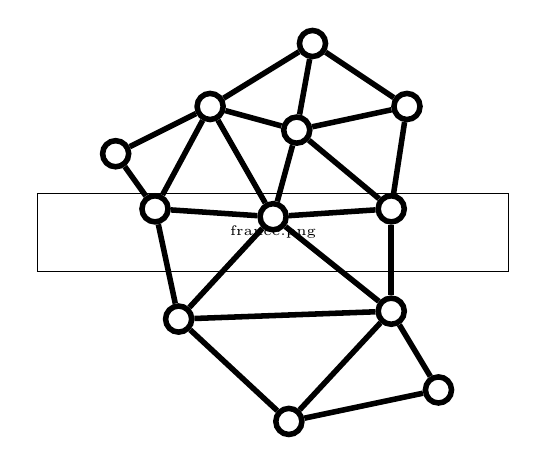
\begin{tikzpicture} 
\draw (0,0) node {\pgfuseimage{france}}; 

%\draw (-3,-3) grid (3,3) ; 
\foreach[count=\k] \x/\y in {-2/1,
                             -0.8/1.6,
                             0.5/2.4,
                             1.7/1.6,
                             1.5/0.3,
                             0.3/1.3,
                             0/0.2,
                             -1.2/-1.1,
                             0.2/-2.4,
                             1.5/-1,
                             2.1/-2,
                             -1.5/0.3} 
   \draw (\x,\y) node[line width=2pt,draw,fill=white,circle] (a\k) {} ;
 \foreach \i/\j in {1/2,1/12,
                    2/3,2/6,2/7,2/12,
                    3/4,3/6,
                    4/5,4/6,
                    5/6,5/7,5/10,
                    6/7,
                    7/8,7/10,7/12,
                    8/9,8/10,8/12,
                    9/10,9/11,
                    10/11}
   \draw[line width=2pt] (a\i) -- (a\j) ;
\end{tikzpicture} 
%-------------------------------------------------------------------------------
\caption{\label{fig:1:france}Exemple de graphe colorié : le graphe des régions métropolitaines françaises (hors Corse). Deux régions sont reliées par une arête dans le graphe si et seulement si elles sont voisines. Deux régions voisines sont de couleurs différentes. }
\end{figure} 
%-------------------------------------------------------------------------------

Un graphe $G$ est dit $k$-coloriable s'il admet un coloriage avec au plus $k$ couleurs. Un graphe est dit colorié s'il est muni d'un coloriage. Un exemple de graphe colorié est donné sur la figure \ref{fig:1:france} ci-dessus. 
%-------------------------------------------------------------------------------
Le \emph{nombre chromatique} d'un graphe non-orienté $G$, noté $\chi(G)$, est le nombre minimal $k$ tel que $G$ est $k$-coloriable. Cet énoncé porte sur le calcul des nombres chromatiques et de coloriages. 
%-------------------------------------------------------------------------------
\subsection*{Représentation des graphes étiquetés}
%-------------------------------------------------------------------------------
On se fixe dans cet énoncé une représentation des graphes par matrices d'adjacence. On se fixe également comme convention que les étiquetages des graphes sont tous à valeurs entières. L'étiquetage d'un graphe sera donné par un tableau d'entiers. On utilisera les types Ocaml suivants : 
\begin{lstlisting} 
type graphe = bool array array;;
type etiquetage = int array ;; 
\end{lstlisting}
%-------------------------------------------------------------------------------
Il n'est pas nécessaire de forcer les types : on considérera qu'ils sont confondus dans la suite du sujet. Ainsi, si une fonction @graphe -> int@ est attendue, alors une fonction @bool array array -> int@ convient. 

Un graphe non-orienté $G = (S,A)$ avec $S= \{ 0, \dots, n-1\}$ est représenté par une valeur @gphe@ de type @graphe@ telle que pour tous sommets $i,j \in S$, on ait @gphe.(i).(j) = true@ si et seulement si $(i,j) \in A$. Le graphe $G$ étant supposé non-orienté, on a alors également par symétrie @gphe.(j).(i) = true@. Pour un étiquetage @etiq@ de @gphe@, l'étiquette du sommet @i@ de @gphe@ est donnée par @etiq.(i)@. 

\newpage
%-------------------------------------------------------------------------------
\subsection*{Fonctions OCaml}
%-------------------------------------------------------------------------------
En plus des fonctionnalités de base du langage Ocaml, le/la candidat.e pourra utiliser les fonctions suivantes sans les programmer : 
\begin{itemize} 
    \item @List.length : 'a list -> int@ \\
    @List.length l@ renvoie la longueur de @l@.
    \item @Array.of_list : 'a list -> 'a array@ \\
    @Array.of_list l@ renvoie un vecteur @t@ de même longueur que @l@, qui contient les mêmes éléments que @l@ et dans le même ordre.
    \item @range : int -> int array@\\ 
    @range n@ renvoie le vecteur @[|0, ..., n-1|]@.
\end{itemize}
%-------------------------------------------------------------------------------
%-------------------------------------------------------------------------------
%-------------------------------------------------------------------------------
\section{Coloriage} 
%-------------------------------------------------------------------------------
%-------------------------------------------------------------------------------
%-------------------------------------------------------------------------------
\begin{Exercise}\it
Indiquer, pour chacun des graphes suivants, s'il est colorié.
\end{Exercise} 
%-------------------------------------------------------------------------------
\begin{Answer}
Le premier graphe admet deux sommets adjacent qui ont la même couleur ; l'étiquetage proposé n'est pas un coloriage. 

Le second est colorié car l'étiquetage proposé est un 3-coloriage.
\end{Answer}
%-------------------------------------------------------------------------------
%-------------------------------------------------------------------------------
\begin{center}
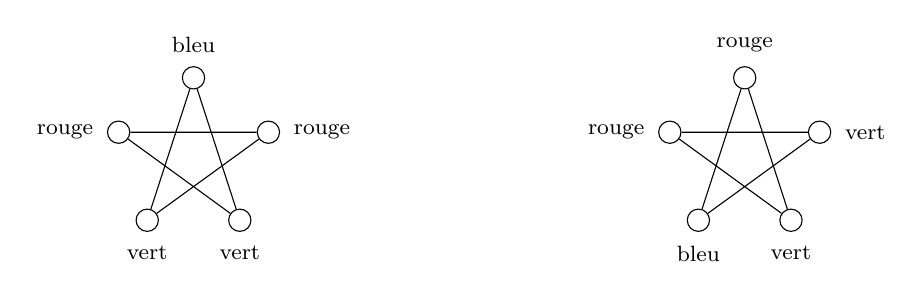
\begin{tikzpicture}
\foreach[count=\k] \c/\pos in {bleu/above,vert/below,rouge/right,rouge/left,vert/below}
    \draw ({90+(\k-1)*360*2/5}:1cm) node [draw,circle,inner sep=1mm] (a\k)  {} node [\pos=2mm] {\footnotesize \c};
\draw (a1) -- (a2) -- (a3) -- (a4) -- (a5) -- (a1);
\begin{scope}[xshift=7cm]
\foreach[count=\k] \c/\pos in {rouge/above,bleu/below,vert/right,rouge/left,vert/below}
    \draw ({90+(\k-1)*360*2/5}:1cm) node [draw,circle,inner sep=1mm] (a\k)  {} node [\pos=2mm] {\footnotesize \c};
\draw (a1) -- (a2) -- (a3) -- (a4) -- (a5) -- (a1);  
\end{scope}
\end{tikzpicture}
\end{center}
%-------------------------------------------------------------------------------
\begin{Exercise}\it 
Donner le nombre chromatique, ainsi qu'un exemple de coloriage correspondant, pour le \emph{graphe de Petersen} représenté figure \ref{fig:2:petersen} 
\end{Exercise}  
%-------------------------------------------------------------------------------
\begin{Answer}
Le graphe contient des cycles de longueur impaire, par exemple (0, 4, 3, 9, 6) : il n'est pas 2-coloriable. En effet il faudrait que les couleurs soient alternées dans le cycle et on arriverait à deux couleurs égales pour les sommets 0 et 6 qui sont reliés.

Par contre il est 3-coloriable :

\begin{center}
\begin{tikzpicture}
\foreach \n/\p/\a/\c/\k in {0/5/0/R/V, 4/8/1/B/R, 3/7/2/V/R, 9/2/3/R/B, 6/1/4/V/B}
  {\node[state] (S\n) at (90+\a*72:3) {\n, \c};
   \node[state] (S\p) at (90+\a*72:1.5) {\p, \k};
   \draw (S\n) --(S\p);};
\draw (S0) -- (S4) -- (S3) -- (S9) -- (S6) -- (S0);
\draw (S5) -- (S7) -- (S1) -- (S8) -- (S2) -- (S5);
\end{tikzpicture}
\end{center}
\end{Answer}
%-------------------------------------------------------------------------------
%-------------------------------------------------------------------------------
\begin{figure}[h]
\centering
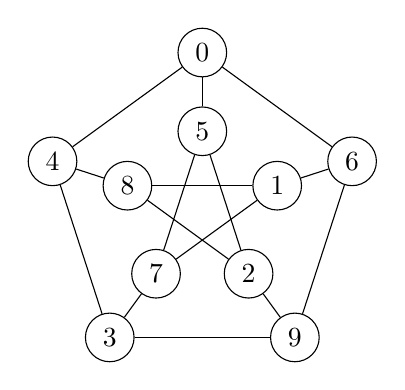
\begin{tikzpicture}[every node/.style={draw,circle}]
\foreach[count=\k] \v in {5,7,1,8,2}
   \draw ({90+(\k-1)*360*2/5}:1cm) node (a\k) {\v}; 
\foreach[count=\k] \v in {0,3,6,4,9}
   \draw ({90+(\k-1)*360*2/5}:2cm) node (b\k) {\v}; 
\foreach \k/\a/\b in {1/2/4,2/3/5,3/4/1,4/5/2,5/1/3} {
   \draw (a\k) -- (a\a) ; 
   \draw (a\k) -- (b\k) ; 
   \draw (b\k) -- (b\b) ;}
\end{tikzpicture} 
%-------------------------------------------------------------------------------
\caption{\label{fig:2:petersen} Le graphe de Petersen, de sommets 0, \dots, 9.}
\end{figure}
%-------------------------------------------------------------------------------
La vérification de la propriété de coloriage est le problème suivant.
\begin{itemize} 
    \item \emph{Entrée} : un graphe $G$ et un étiquetage $L$ de $G$. 
    \item \emph{Exercise}  : $L$ est-il un coloriage de $G$ ? 
\end{itemize}
%-------------------------------------------------------------------------------
\begin{Exercise} \it
Écrire une fonction @est_col : graphe -> etiquetage -> bool@, telle que @est_col gphe etiq@ renvoie @true@ si et seulement si @etiq@ est un coloriage de @gphe@. Dans le cas où la taille de l'étiquetage est strictement inférieure au nombre de sommets du graphe, la fonction renvoie @false@. On demande une complexité quadratique en le nombre de sommets du graphe. 
\end{Exercise}  
%-------------------------------------------------------------------------------
\begin{Answer}
\begin{lstlisting}
let est_col gphe etiq =
   let n = Array.length gphe in
   let p = Array.length etiq in
   let coloriable = ref true in
   if n > p
   then coloriable := false
   else for i = 0 to (n-2) do
           for j = (i+1) to (n-1) do
              if gphe.(i).(j) && etiq.(i) = etiq.(j)
              then coloriable := false done done;
   !coloriable;;
\end{lstlisting}
\end{Answer}
%-------------------------------------------------------------------------------
%-------------------------------------------------------------------------------
\begin{Exercise}[label=q:chromaEXP] \it
Démontrer que le calcul du nombre chromatique d'un graphe peut s'effectuer en temps exponentiel en le nombre de sommets. 
\end{Exercise}  
%-------------------------------------------------------------------------------
\begin{Answer}
Un graphe de $n$ sommet possède un $n$-coloriage, il suffit de donner une couleur distincte à chaque sommet.

Pour tester son nombre chromatique il suffit de tester, pour $k$ variant de 2 à $n-1$ s'il admet un coloriage à $k$ couleurs. 

Pour cela on peut tester tous les coloriages : il y en a $k^n$.

La complexité est exponentielle car elle est majorée par 
\[An^2\left(\sum_{k=2}^{n-1} k^n\right) \le An^2.n.n^n= A2^{(n+3)\log_2(n)} \le B2^{n^2}\]
\end{Answer}
%-------------------------------------------------------------------------------
%-------------------------------------------------------------------------------
%-------------------------------------------------------------------------------
\section{2-coloriage}
%-------------------------------------------------------------------------------
%-------------------------------------------------------------------------------
%-------------------------------------------------------------------------------
Nous avons vu à la question \ref{q:chromaEXP} que le calcul du nombre chromatique peut s'effectuer en temps exponentiel en le nombre de sommets du graphe. Dans le cas général, on ne sait aujourd'hui pas faire mieux. Pour obtenir de meilleures bornes de complexité, il faut donc se limiter à des sous-problèmes. On considère dans cette partie le cas du $2$-coloriage. 

\medskip

\textbf{Graphe biparti.} Un graphe $G$ est \emph{biparti} lorsque l'ensemble de ses sommets $S$ peut être divisé en deux sous-ensembles disjoints $T$ et $U$, tels que chaque arête a une extrémité dans $T$ et l'autre dans $U$. 
%-------------------------------------------------------------------------------
%-------------------------------------------------------------------------------
\begin{Exercise} \it
Démontrer qu'un graphe $G$ est biparti si et seulement s'il est $2$-coloriable. 
\end{Exercise}  
%-------------------------------------------------------------------------------
\begin{Answer}
Si $G$ est biparti, alors ses sommets peuvent se diviser en deux sous-ensembles $T$ et $U$. On attribue alors la couleur 1 aux sommets de $T$, et 2 aux sommets de $U$. La propriété de coloration est alors instantanément vérifiée.

Inversement, si $G$ possède une 2-coloration, alors on peut appeler $T$ les sommets recevant la couleur 1 et $U$ les sommets recevant la couleur 2. Aucune arête ne peut relier deux sommets de même couleur  et les arêtes vont donc d'un sommet de $T$ vers un sommet de $U$. 
\end{Answer}
%-------------------------------------------------------------------------------
%-------------------------------------------------------------------------------
On se propose de programmer la vérification de la $2$-colorabilité des graphes en procédant comme suit. On effectue un parcours du graphe en profondeur au cours duquel on construit une $2$-coloration du graphe. On se donne pour ce faire trois étiquettes, disons $-1$, $0$ et $1$. 

L'étiquetage est initialisé à $-1$ pour tous les sommets, et on teste la $2$-colorabilité avec $0$ et $1$. Le principe de l'algorithme est le suivant :
\begin{enumerate}
    \item \label{item:init}On choisit un sommet $s$ d'étiquette $-1$.
    \item On colorie les sommets rencontrés lors du parcours en profondeur à partir de $s$, en alternant entre les couleurs $0$ et $1$ à chaque incrémentation de la profondeur, et en vérifiant si les sommets déjà coloriés rencontrés sont d'une couleur compatible. 
    \item Enfin, s'il reste des sommets d'étiquette $-1$, alors on revient au point (\ref{item:init}). 
\end{enumerate}
%-------------------------------------------------------------------------------
%-------------------------------------------------------------------------------
\begin{Exercise} \it 
Écrire une fonction @deux_col : graphe -> etiquetage@ telle que @deux_col gphe@ renvoie un $2$-coloriage de @gphe@ si @gphe@ est $2$-coloriable. Le coloriage utilisera les couleurs $0$ et $1$. On demande une complexité quadratique en le nombre de sommets du graphe. Le comportement de la fonction est laissé au choix du/de la candidat.e lorsque @gphe@ n'est pas $2$-coloriable. 
\end{Exercise}  
%-------------------------------------------------------------------------------
\begin{Answer}
\begin{lstlisting}
let deux_col gphe = 
   let n = Array.length gphe in
   let etiq = Array.make n (-1) in
   let rec explo i k = 
      etiq.(i) <- k;
      for j = 0 to n-1 do
          if gphe.(i).(j) && etiq.(j) = -1 
          then explo j (1-k) done in
   for i = 0 to n-1 do
      if etiq.(i) = -1 
      then explo i 0 done;
   etiq;; 
\end{lstlisting}

Ici, si le graphe n'est pas 2-coloriable, alors le programme renvoie une coloration fausse (on ne détecte pas les erreurs si le sommet j est déjà colorié). 

Le programme \texttt{explo} ne peut être lancé qu'une seule fois par sommet au maximum, et sa complexité est en $O(n)$. On arrive donc à une complexité en $O(n^2)$ dans le pire des cas. 
\end{Answer}
%-------------------------------------------------------------------------------
%-------------------------------------------------------------------------------
%-------------------------------------------------------------------------------
\section{Algorithmes gloutons} 
%-------------------------------------------------------------------------------
%-------------------------------------------------------------------------------
%-------------------------------------------------------------------------------
Dans cette partie, nous allons étudier deux algorithmes permettant de colorier un graphe en temps polynomial, mais donnant en général un coloriage sous-optimal : le coloriage obtenu peut dans certains cas utiliser plus de couleurs que le coloriage optimal. 

\medskip

Ces deux algorithmes prennent en paramètre un ordre sur les sommets du graphe, que l'on appellera \emph{ordre de numérotation}. 

Par exemple, $1<3<4<0<2<6<5<9<8<7$ et 

$0<7<2<5<4<6<8<1<3<9$ sont deux ordres de numérotation des sommets du graphe de Petersen (figure \ref{fig:2:petersen}).

\medskip

Pour un graphe @gphe@ à $n$ sommets, on implémente un ordre de numérotation de ses sommets par un tableau @num@ de $n$ valeurs entières, tel que @num.(k) = j@ si et seulement si le sommet @j@ apparaît en $(k+1)$-ème position dans l'ordre. 

\medskip

Nous commençons par l'\emph{algorithme glouton} de coloriage. Cet algorithme construit un coloriage $L$ d'un graphe $G$ en utilisant au plus $d(G)+1$ couleurs. Son principe est le suivant :

On parcourt la liste des sommets du graphe, dans l'ordre de numérotation des sommets donné. Pour chaque sommet $s$ parcouru : 
\begin{enumerate}
    \item On calcule l'ensemble $C(s) = \{ L(t) | t \in V(s) \}$ des couleurs déjà données aux voisins de $s$. 
    \item On cherche le plus petit entier naturel $c$ qui n'appartient pas à $C(s)$. 
    \item On pose $L(s) = c$.
\end{enumerate} 
%-------------------------------------------------------------------------------
%-------------------------------------------------------------------------------
\begin{Exercise}\it 
 Considérons le graphe de Petersen (figure \ref{fig:2:petersen}) et les deux ordres de numérotation :
 
@num1 = [|1;3;4;0;2;6;5;9;8;7|]@ et @num2 = [|0;7;2;5;4;6;8;1;3;9|]@. 

Donner les coloriages obtenus par l'algorithme glouton décrit ci-dessus pour le graphe de Petersen et chacun de ces deux ordres de numérotation, ainsi que les nombres de couleurs correspondants. 
\end{Exercise}  
%-------------------------------------------------------------------------------
\begin{Answer}
Avec le premier ordre, on trouve comme colorations pour les sommets : $(0;0;0;0;1;1;1;2;2;2)$, donc trois couleurs. 

Avec le second, on trouve comme colorations : $(0;3;0;2;1;1;1;0;2;3)$, donc quatre couleurs.
\end{Answer}
%-------------------------------------------------------------------------------
%-------------------------------------------------------------------------------
\begin{Exercise}\it 
Écrire une fonction  @min_couleur_possible : graphe -> etiquetage -> int -> int @ telle que pour un graphe @gphe@ à $n$ sommets, un étiquetage @etiq@ à valeurs dans $\{-1,\dots,n-1\}$, et pour un sommet @s@ de @gphe@, l'appel de @min_couleur_possible gphe etiq s@ renvoie le plus petit entier naturel n'appartenant pas à l'ensemble $\{$ @etiq.(t)@ $|$ @t@ $ \in V($ @s@ $) \}$. 

On demande une complexité en $O(n)$. 
\end{Exercise}  
%-------------------------------------------------------------------------------
\begin{Answer}
\begin{lstlisting}
let min_couleur_possible gphe etiq s =
   let n = Array.length gphe in
   let coul = Array.make n false in
   for i = 0 to (n-1) do
      if gphe.(s).(i) && etiq.(i) <> -1
      then coul.(etiq.(i)) <- true done;
   let c = ref 0 in
   while coul.(!c) do c := !c + 1 done;
   !c;;
\end{lstlisting}
\end{Answer}
%-------------------------------------------------------------------------------
%-------------------------------------------------------------------------------
\begin{Exercise}\it 
 Écrire une fonction @glouton : graphe -> int array -> etiquetage@, telle que, pour un graphe @gphe@ et un ordre de numérotation @num@ de ses sommets, @glouton gphe num@ renvoie le coloriage glouton de @gphe@, avec au plus $d+1$ couleurs, où $d$ est le degré de @gphe@. On demande une complexité en $O(n^2)$, où $n$ est le nombre de sommets de @gphe@. 

Dans le cas où le tableau @num@ contient autre chose qu'un ordre de numérotation des sommets de @gphe@, le résultat de la fonction est laissé au choix du/de la candidat.e.
\end{Exercise}  
%-------------------------------------------------------------------------------
\begin{Answer}
\begin{lstlisting}
let glouton gphe num =
   let n = Array.length gphe in
   let coul = Array.make n (-1) in
   for i = 0 to (n-1) do
      let k = num.(i) in
      coul.(k) <- min_couleur_possible gphe coul k done;
  coul;;
\end{lstlisting}
\end{Answer}
%-------------------------------------------------------------------------------
%-------------------------------------------------------------------------------
\begin{Exercise}\it 
 Montrer que l'algorithme de coloriage glouton construit toujours un coloriage, et que ce coloriage utilise au plus $d+1$ couleurs, où $d$ est le degré du graphe en entrée. 
\end{Exercise}  
%-------------------------------------------------------------------------------
\begin{Answer}
La fonction \texttt{min\_couleur\_possible} renvoie une couleur qui n'a pas été affectée aux voisins du sommet passé en paramètre.
Lorsqu'une couleur est affectée à un sommet elle ne pourra plus être affectée aux voisins qui suivent dans l'ordre de numération.
De plus chaque sommet reçoit une couleur lorsque \texttt{num} est un ordre de numération.

On a bien construit un coloriage du graphe.

\medskip

Dans l'algorithme glouton chaque sommet est colorié par une couleur non employée par ses voisins déjà coloriés, comme il admet au plus $d(G)$ voisins, l'ensemble $\{0, 1, \ldots, d(G)\}$ contient au moins une valeur non atteinte par les voisins. La couleur choisie est donc dans cet ensemble de cardinal $1+d(G)$ à chaque étape donc la coloration construite admet au plus $d(G)+1$ couleurs.
\end{Answer}
%-------------------------------------------------------------------------------
%-------------------------------------------------------------------------------
\begin{Exercise} [label=q:ordreoptimal]\it 
Soit $G$ un graphe. Montrer que pour tout coloriage $L$ de $G$, il existe un ordre de numérotation des sommets tel que le coloriage glouton $L'$ associé vérifie $L'(s) \leq L(s)$ pour tout sommet $s$ de $G$. En déduire qu'il existe une numérotation des sommets telle que l'algorithme glouton renvoie un coloriage optimal. 
\end{Exercise}  
%-------------------------------------------------------------------------------
\begin{Answer}
Soit $L$ un coloriage de $G$. On considère une numération des sommets qui les classe par numéro de couleur croissante.

Comme deux sommets de même couleur ne sont pas adjacents, lors de l'appel de \texttt{min\_couleur\_possible} les seuls sommets voisins de $s$ qui seront considérés auront une couleur strictement inférieure à celle de $s$, $L(s)$. La couleur choisie, $L'(s)$, ne pourra donc pas être strictement supérieure à $L(s)$ : on a $L'(s) \le L(s)$ pour tout $s$.

Si on part d'un coloriage optimal pour construire la numération des sommets on aboutit donc à un coloriage dont le maximum est majoré par celui du coloriage optimal : ce sera donc aussi un coloriage optimal.
\end{Answer}
%-------------------------------------------------------------------------------
%-------------------------------------------------------------------------------
Les questions 7 à 11 indiquent que l'efficacité de l'algorithme glouton est en grande partie dépendante de l'ordre dans lequel on choisit de parcourir les sommets du graphe. L'ordre correspondant à la représentation choisie du graphe (dans notre cas les indices de la matrice d'adjacence, c'est-à-dire la permutation identité) est le plus simple à calculer, mais a peu de chances d'être efficace. A contrario, on pourrait essayer de déterminer l'ordre optimal, dont on a prouvé l'existence à la question \ref{q:ordreoptimal}, mais cela n'apporterait aucun bénéfice vis-à-vis de la complexité temporelle.

Une alternative est donnée par l'optimisation de Welsh-Powell. L'idée est de parcourir l'ensemble des sommets du graphe par ordre de degré décroissant. Le tri des sommets par degré décroissant ne prend pas plus de temps que le parcours glouton, mais permet d'obtenir un algorithme raisonnablement efficace en pratique. 
%-------------------------------------------------------------------------------
%-------------------------------------------------------------------------------
\begin{Exercise} \it 
Écrire une fonction @tri_degre : graphe -> int array@, qui calcule le tableau des sommets d'un graphe trié par ordre décroissant de leurs degrés. En déduire une fonction @welsh_powell : graphe -> etiquetage@ qui implémente l'optimisation de Welsh-Powell, et justifier le choix de votre algorithme de tri pour la fonction @tri_degre@. 
\end{Exercise}  
%-------------------------------------------------------------------------------
\begin{Answer}
Comme l'algorithme \texttt{glouton} est de complexité quadratique on peut choisir un algorithme lui-même quadratique pour construire une numération des sommets sans augmenter la complexité.

On commence par construire un tableau avec les degrés.
\begin{lstlisting}
let degres gphe =
   let n = Array.length gphe in
   let deg = Array.make n 0 in
   for i = 0 to (n-1) do 
      for j = 0 to (n-1) do
         if gphe.(i).(j) 
         then deg.(i) <- deg.(i) + 1 done done;
   deg;;           
\end{lstlisting}

Les outils utilisés ensuite (dont \texttt{range})

\begin{lstlisting}
let echanger tab i j =
   let temp = tab.(i) in
   tab.(i) <- tab.(j);
   tab.(j) <- temp;;
    
let range n = 
   Array.init n (fun x -> x);;        
\end{lstlisting}

La création de la numération suit la méthode du tri par sélection
\begin{lstlisting}
let tri_degre gphe =
   let n = Array.length gphe in
   let deg = degres gphe in
   let num = range n in
   for i = 0 to (n-2) do
      let max = ref i in
      let deg_max = ref deg.(num.(i)) in
      for j = (i+1) to (n-1) do
      let d =  deg.(num.(j)) in
         if d > !deg_max
         then (max := j; deg_max := d) done;
      echanger num i !max done;
   num;;
\end{lstlisting}

Il suffit alors de tout rassembler.
\begin{lstlisting}
let welsh_powell gphe =
    glouton gphe (tri_degre gphe);;
\end{lstlisting}
\end{Answer}
%-------------------------------------------------------------------------------
%-------------------------------------------------------------------------------
%-------------------------------------------------------------------------------
\section{Algorithme de Wigderson} 
%-------------------------------------------------------------------------------
%-------------------------------------------------------------------------------
%-------------------------------------------------------------------------------
Considérons un graphe $G$ avec $n$ sommets. Supposons que $G$ soit $3$-coloriable, mais que l'on ait cette information sans pour autant effectivement disposer d'un $3$-coloriage de $G$. Trouver un $3$-coloriage de $G$ pourrait prendre un temps exponentiel en $n$. 

L'algorithme de Wigderson permet, pour un graphe $G$ supposé $3$-coloriable, de trouver en temps polynomial en $n$ un coloriage de $G$ en au plus $K\sqrt{n}$ couleurs couleurs où $K$ est une constante.

Cet algorithme repose sur la propriété établie dans la question qui suit. 
%-------------------------------------------------------------------------------
%-------------------------------------------------------------------------------
\begin{Exercise}\it Soit $k >0$. Montrer que si $G$ est $(k+1)$-coloriable, alors pour tout sommet $s$ de $G$ le sous-graphe induit par $V(s)$ est $k$-coloriable. 
\end{Exercise}  
%-------------------------------------------------------------------------------
\begin{Answer}
Supposons que le graphe $G$ est $(k+1)$-coloriable, et soit $s$ un de ses sommets. On considère une $(k+1)$-coloration de $G$. Alors aucun sommet de $V(s)$ n'est de la même couleur que $s$ (ce serait contradictoire). Sur le sous-graphe induit par $V(s)$, cette coloration reste valide, et n'utilise donc que $k$ couleurs au maximum (celle de $s$ n'est pas employée).  
\end{Answer}
%-------------------------------------------------------------------------------
%-------------------------------------------------------------------------------
Voici le principe de l'algorithme de Wigderson. Soit $G$ un graphe à $n$ sommets, et tel que $G$ est $3$-coloriable.
\begin{enumerate}
    \item On se donne comme couleur initiale $c=0$. 
    \item Pour chaque sommet $s$ de $G$ pas encore colorié et ayant au moins $\sqrt{n}$ voisins pas encore coloriés : \begin{enumerate}
        \item On $2$-colorie, avec les couleurs $c$ et $c+1$, le sous-graphe induit par l'ensemble des voisins de $s$ pas encore coloriés. 
        \item On incrémente $c$ du nombre de couleurs utilisées en (a). 
        \end{enumerate}
    \item Enfin, on utilise l'algorithme glouton (avec un ordre de numérotation quelconque) pour colorier, avec des couleurs supérieures ou égales à $c$, le sous-graphe induit par l'ensemble des sommets par encore coloriés. 
\end{enumerate}
%-------------------------------------------------------------------------------
%-------------------------------------------------------------------------------
\begin{Exercise} \label{q:pptewigderson}\it Montrer que l'algorithme de Wigderson appliqué à un graphe $3$-coloriable construit toujours un coloriage, et que ce coloriage utilise un nombre de couleur en $O(\sqrt{n})$, où $n$ est le nombre de sommets du graphe. 
\end{Exercise}  
%-------------------------------------------------------------------------------
\begin{Answer}
Fixons les notations.

On pose $G_0=G$ de taille $n$.

L'étape $(a)$ se décompose en étapes.
\begin{enumerate}[noitemsep]
    \item Si $G_i$ admet un sommet de degré supérieur à $\sqrt n$,
    \item on choisit un tel sommet, $s_i$, par exemple celui de degré maximum,
    \item on colorie avec les couleurs $2i$ et $2i+1$ $V(s_i)$, ce qui est possible d'après la question précédente. En effet $G_i$ est induit d'un graphe 3-coloriable donc est 3-coloriable d'où $V(s_i)$ est 2-coloriable.
    \item On définit $G_{i+1}$ comme le graphe induit de $G_i$ en enlevant les sommets appartenant à $V(s_i)$.
\end{enumerate}
Après au plus $\sqrt n$ itérations $G_p$ n'admet plus de sommet de degré supérieur à $\sqrt n$ et on le colorie par l'algorithme glouton.

On a ainsi partitionné l'ensemble des sommets : $S = S_0\cup S_1\cup\cdots S_p$,

où $S_i=V(s_i)$ pour $i<p$ et $S_p$ est l'ensemble des sommets de $G_p$.

Chaque $S_i$ admet un coloriage : 
\begin{enumerate}[noitemsep]
    \item pour $i<p$,  $V(s_i)$ est colorié par $2i$ et $2i+1$,
    \item $G_p$ est colorié par $q$ couleurs qui sont supérieures ou égales à $2p$. 
    
    De plus, d'après la question {\bf 10}, on a $q\le\sqrt n+1$.
\end{enumerate}
Comme chaque partie est coloriée par des couleurs distinctes on obtient un coloriage de $G$ avec $2p+q$ couleurs qui vérifient $2p+q \le 2\sqrt n + \sqrt n +1 = {\cal O}\bigl(\sqrt n\bigr)$.
\end{Answer}
%-------------------------------------------------------------------------------
%-------------------------------------------------------------------------------
Nous allons maintenant implémenter cet algorithme. 

Commençons par programmer quelques fonctions auxiliaires simples. 
%-------------------------------------------------------------------------------
%-------------------------------------------------------------------------------
\begin{Exercise}\it Écrire une fonction @sous_graphe : graphe -> int array -> graphe@ telle que pour 

@gphe : graphe@ et @sg : int array@, si @sg@ est à valeurs dans $\{0, \dots, $ @Array.length gphe - 1@$\}$ et sans répétition, alors @sous_graphe gphe sg@ renvoie la matrice d'adjacence du graphe de sommets $\{0, \dots, $ @Array.length sg - 1@ $\}$, et qui a une arête entre les sommets @s@ et @t@ si et seulement si \\ @gphe.(sg.(s)).(sg.(t)) = true@.

Dans le cas où @sg@ a des valeurs hors de $\{0, \dots, $ @Array.length gphe - 1@ $\}$, ou a des répétitions, le comportement de la fonction @sous_graphe@ est laissé au choix du/de la candidat.e. 
\end{Exercise}  
%-------------------------------------------------------------------------------
\begin{Answer}
\begin{lstlisting}
let sous_graphe gphe sg =
   let p = Array.length sg in
   let ss_gphe = Array.make_matrix p p false in
   for i = 0 to (p-1) do
      let si = sg.(i) in
      for j = 0 to (p-1) do
         let sj = sg.(j) in
         ss_gphe.(i).(j) <- gphe.(si).(sj) done done;
   ss_gphe;;
\end{lstlisting}
\end{Answer}
%-------------------------------------------------------------------------------
%-------------------------------------------------------------------------------
Nous nous proposons d'utiliser pour les étiquetages la même convention que précédemment : on se donnera un étiquetage @etiq :etiquetage@ de longueur @Array.length gphe@, initialisé à $-1$, et que l'on mettra à jour au fur et à mesure de l'algorithme. 
%-------------------------------------------------------------------------------
%-------------------------------------------------------------------------------
\begin{Exercise}\it Écrire une fonction @voisins_non_colories : graphe -> etiquetage -> int -> int list@ telle que @voisins_non_colories gphe etiq s@ renvoie la liste des voisins @t@ de @s@ non étiquetés,
c'est-à-dire tels que @etiq.(t) = -1@. 

En déduire une fonction @degre_non_colories : graphe -> etiquetage -> int -> int@ telle que @degre_non_colories gphe etiq s@ renvoie le nombre de voisins @t@ de @s@ . 
\end{Exercise}  
%-------------------------------------------------------------------------------
\begin{Answer}
\begin{lstlisting}
let voisins_non_colories gphe etiq s =
   let n = Array.length gphe in
   let vnc = ref [] in
   for j = 0 to (n-1) do
      if gphe.(s).(j) && etiq.(j) = -1
      then vnc := j :: !vnc done;
   !vnc;;
  
let degre_non_colories gphe etiq s =
    List.length (voisins_non_colories gphe etiq s);;
\end{lstlisting}
\newpage
\end{Answer}
%-------------------------------------------------------------------------------
%-------------------------------------------------------------------------------
\begin{Exercise}\it Écrire une fonction @non_colories : graphe -> etiquetage -> int list@ telle que @non_colories gphe etiq@ renvoie la liste des sommets @s@ de @gphe@ non étiquetés.
\end{Exercise}  
%-------------------------------------------------------------------------------
\begin{Answer}
\begin{lstlisting}
let non_colories gphe etiq =
   let n = Array.length gphe in
   let nc = ref [] in
   for i = 0 to (n-1) do
      if etiq.(i) = -1
      then nc := i :: !nc done;
   !nc;;
\end{lstlisting}
\end{Answer}
%-------------------------------------------------------------------------------
%-------------------------------------------------------------------------------
Nous disposons maintenant de toutes les briques nécessaires à l'implémentation de l'algorithme de Wigderson. 
%-------------------------------------------------------------------------------
%-------------------------------------------------------------------------------
\begin{Exercise}\it Écrire une fonction @wigderson : graphe -> etiquetage@ telle que si @gphe@ est $3$-coloriable, alors @wigderson gphe@ renvoie un coloriage de gphe obtenu par l'algorithme de Wigderson décrit plus haut. On demande une complexité polynomaile en le nombre de sommets de @gphe@. De plus, les propriétés sur le coloriage établies à la question \ref{q:pptewigderson} devront être respectées et justifiées. 

Le comportement de la fonction est laissé au choix du/de la candidat.e lorsque @gphe@ n'est pas $3$-coloriable.
\end{Exercise}  
%-------------------------------------------------------------------------------
\begin{Answer}

Pour ne pas écrire un programme démesurément long, on sort quelques fonctions. 

La première détermine le degré en sommets non coloriés maximal. Le test de majoration de $\sqrt n$ est renvoyé par le type optionnel : la fonction renvoie \texttt{None} s'il n'existe pas de sommets avec suffisamment de voisins non coloriés et sinon elle renvoie un sommet $k$ vérifiant cette proprité sous la forme \texttt{Some k}.
\begin{lstlisting}
let sous_degre_maximum gphe etiq =
   let n = Array.length gphe in
   let r = int_of_float (sqrt (float_of_int n)) in
   let deg_max = ref (degre_non_colories gphe etiq 0) in 
   let ind_max = ref 0 in
   for i = 1 to (n-1) do
      let d = degre_non_colories gphe etiq i in
      if  d > !deg_max
      then (deg_max := d; ind_max := i) done;
   if !deg_max > r then Some !ind_max else None;;
\end{lstlisting}

La seconde modifie le tableau des couleurs (\texttt{etiq}) à partir des couleurs calculées  (\texttt{ss\_etiq}) pour un sous-graphe  (\texttt{sg}) 
\begin{lstlisting}
let ajouter_couleurs etiq sg ss_etiq couleur=
   let p = Array.length sg in
   for i = 0 to (p-1) do
      etiq.(sg.(i)) <- ss_etiq.(i) + couleur done;;
\end{lstlisting}

Le programme consiste alors à répéter la recherche de sommets avec suffisamment de voisins non coloriés tant qu'il en existe.
\begin{lstlisting}
let wigderson g =
   let n = Array.length g in
   let e = Array.make n (-1) in
   let c = ref 0 in
   let rec aux () =
      match sous_degre_maximum g e with
      |None -> let nc = Array.of_list (non_colories g e) in
               let sg = sous_graphe g nc in
               let se = glouton sg (range (Array.length sg)) 
               in ajouter_couleurs e nc se !c
      |Some i -> let nc = Array.of_list (voisins_non_colories g e i) in
                 let sg = sous_graphe g nc in
                 let se = deux_col sg in
                 ajouter_couleurs e nc se !c;
                 c := !c + 2;
                 aux ()
   in aux (); 
   e;;
\end{lstlisting}

Toutes les fonctions auxiliaires sont de complexité polynomiale en la taille du graphe et elles sont appelées au plus $\sqrt n$ fois : la complexité est polynomiale.

Je ne comprends pas la demande de justification des propriétés, c'est ce qui a été fait à la question {\bf 14}.
\end{Answer}
%-------------------------------------------------------------------------------
%-------------------------------------------------------------------------------
\begin{Exercise}\it  
Comment pourrait-on étendre l'algorithme de Wigderson à des graphes de nombre chromatique connu et strictement supérieur à 3 ? 
\end{Exercise}  
%-------------------------------------------------------------------------------
\begin{Answer}
Comme on sait définir un coloriage dans le cas d'un graphe 3-coloriable on peut poursuivre le raisonnement de manière semblable.

Si un graphe est 4-coloriable, les voisins d'un sommets sont 3-coloriables ; on va donc pouvoir définir un coloriage pour les "gros" voisinages puis conclure par un algorithme glouton.

On considère la propriété ${\cal P}(k)$ : 
on peut définir un coloriage de $A_k.n^{a_k}$ couleurs d'un graphe $k$-coloriable avec $a_k< 1$.

${\cal P}(2)$ est vraie avec $a_2=1$ et $A_2=2$.

${\cal P}(3)$ est vraie avec $a_2=\frac 12$ et $A_3=3$.

On suppose ${\cal P}(k)$ vraie. $G$ est un graphe $k+1$-coloriable.

Pour chaque sommet $s$ de $G$ ayant au moins $n^r$ voisins pas encore coloriés on colorie ceux-ci avec au plus $A_k.n^{a_k}$ couleurs non encore utilisées. On colorie le reste avec au plus $n^r+1$ couleurs non utilisées.

Le nombre de sommets avec plus de $n^r$ voisins est au plus $\frac n{n^r}$ donc on a utilisé au plus
$n^{1-r}.A_k.n^{a_k} + n^r$ couleurs.

On peut choisir $r$ tel que l'expression ci-dessus devienne homogène : $1-r+a_k = r$ donc $r = \frac {1+a_k}2$.

On obtient ainsi un coloriage avec au plus $(A_k+1).n^r$ couleurs.

La récurrence $a_{k+1} = \frac {1+a_k}2$ avec $a_2=0$ donne $a_k=1- 2^{2-k}$. donc 

la propriété ${\cal P}(k)$ est donc vraie avec $A_k=k$ et $a_k = 1- 2^{2-k}$.

\medskip

Dans le calcul ci-dessus on n'a pas tenu compte du fait qu'on appliquait ${\cal P}(k)$ à des graphes de tailles inférieures à $n$. 

Si les tailles auxquelles on applique ${\cal P}(k)$ sont $m_1$, $m_2$, \dots, $m_p$, le nombre de couleurs employées est en fait majoré par
$\displaystyle \sum_{i=1}^p A_k.m_i^{a_k}+n^r$

La fonction $x \mapsto n^{a_k}$ est concave donc $\displaystyle \frac {\sum_{i=1}^p m_i^{a_k}}p\le \left(\sum_{i=1}^p \frac {m_i}p\right)^{a_k}$.

Ainsi $\displaystyle \sum_{i=1}^p A_k.m_i^{a_k}+n^r\le p^{1-a_k} A_k \left(\sum_{i=1}^p  m_i\right)^{a_k} + n^r$.

Comme on a $\displaystyle \sum_{i=1}^p  m_i\le n$ et $p \le n^{1-r}$, le nombre de couleurs utilisées est majoré par

$\displaystyle n^{(1-r)(1-a_k)} A_k n^{a_k} + n^r$.

On choisit $a_{k+1}= r$ tel que $(1-r)(1-a_k)+a_k=r$ d'où $r = \frac 1{2-a_k}$.

$a_2=0$ donne bien $a_3 = \frac 12$.

On calcule ensuite $a_4 = \frac 23$, $a_5 = \frac 34$ et, par récurrence, $a_k = \frac{k-2}{k-1}=1 - \frac 1{k-1}$ qui donne moins de couleurs que la valeurs $1 -2^{2-k}$.
\end{Answer}
%-------------------------------------------------------------------------------
%-------------------------------------------------------------------------------
